\vspace{-1mm}
\section{Method}

\begin{figure}
\vspace{-3mm}
\begin{center}
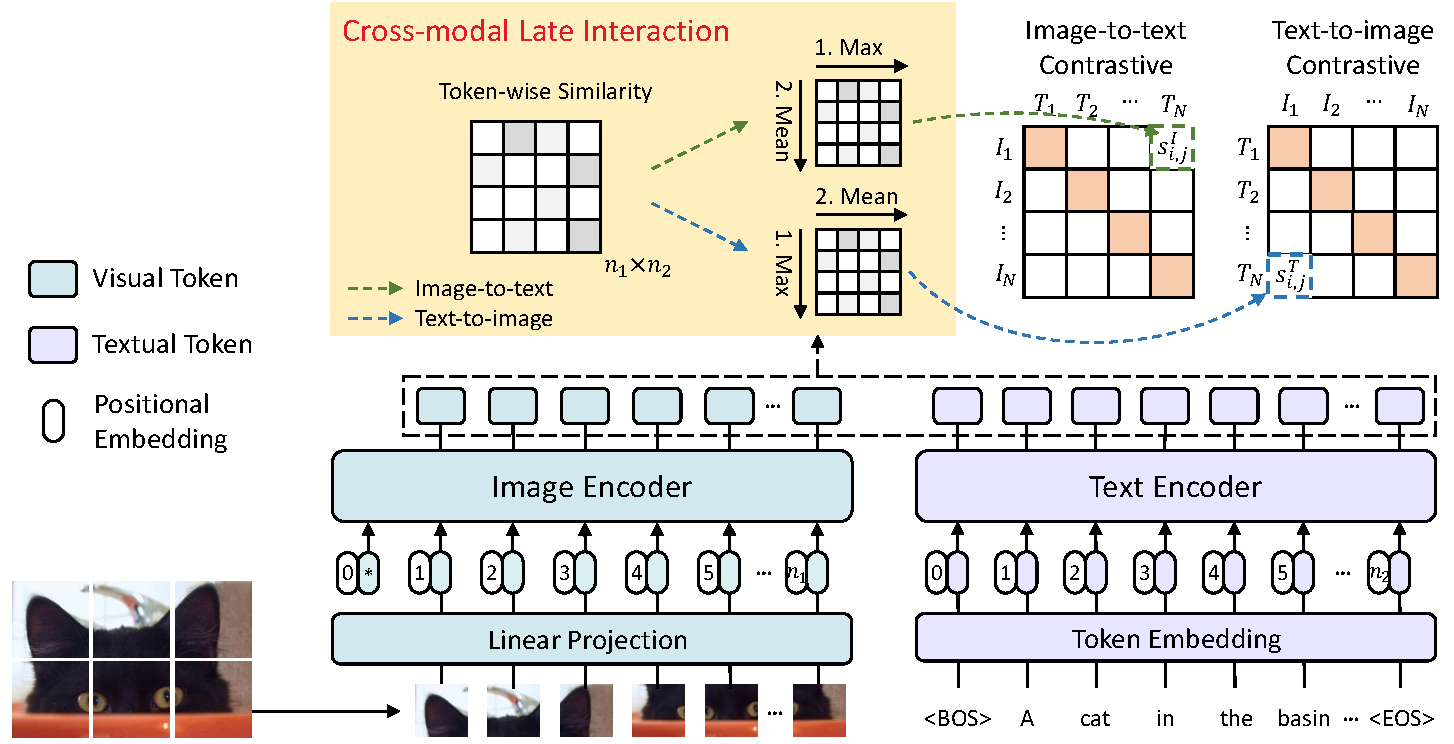
\includegraphics[width=\textwidth]{figures/CLIP_framework.pdf}
\vspace{-6mm}
\caption{Overall architecture of FILIP, a dual-stream model with Transformer-based image and text encoders. On top of the image and text encoders,  the representations of textual tokens and visual tokens are linearly projected to the multi-modal joint space. A novel fine-grained contrastive learning equipped with cross-modal late interaction is proposed, which uses  a  token-wise  maximum  similarity  between visual and textual tokens. }
% patches in the images and words in the sentences.}
\label{fig:framework}
\end{center}
\vspace{-4mm}
\end{figure}

\label{sec:model_overview}

In this paper, we propose a new cross-modal pre-training model that excels in fine-grained interaction between image encoder and text encoder for mining more detailed semantic alignment, named as FILIP, as shown in  Figure \ref{fig:framework}. 
Particularly, FILIP is a dual-stream model with Transformer-based image and text encoders.
For the visual modality, the image encoder is a Vision Transformer \citep{dosovitskiy2020image} which takes the concatenation of an extra [CLS] token embedding and linearly projected image patches as input.
For the textual modality, following \cite{radford2021learning}, we use the lower-cased byte pair encoding (BPE) \citep{sennrich2016neural}
with a vocabulary size of 49,408  to tokenize the text. 
Each text sequence starts with [BOS] token and ends with [EOS] token.
After the word embedding layer, the token embeddings are fed into a modified decoder-only Transformer model as in \citep{radford2019language}. 
On top of the image and text encoders, the representations of textual tokens and visual tokens are linearly projected to the multi-modal common space, and are separately L2-normalized. 
Different from existing dual-stream models (e.g., CLIP and ALIGN) which models cross-modal interaction via only the global features of the entire image and text sequence, 
% we integrate a new interaction layer for learning to better align cross-modal semantics, which is trained with the image captioning loss (see Section \ref{sec:interaction_layer})\footnote{remove?}. 
% Coupled with the interaction layer, we also 
we introduce a novel fine-grained contrastive learning objective equipped with cross-modal late interaction which takes into account the fine-grained interaction between image patches and textual tokens, detailed in Section \ref{sec:late_interaction}.
% \hou{Coupled with this, we also
%  integrate a new interaction layer trained with the image captioning loss to better align cross-modal semantics in Section \ref{sec:interaction_layer})}\footnote{remove?}. 




\vspace{-1mm}
\subsection{Fine-grained Contrastive Learning}
\label{sec:late_interaction}

% \textbf{Preliminary.}
Contrastive representation learning has recently been found to learn better representations than its predictive counterpart 
in both visual \citep{tian2020contrastive} and vision-language cross-modal pre-training  \citep{radford2021learning}.
Under a general formulation of cross-modal contrastive learning \citep{radford2021learning}, we want to learn encoders $f_\theta$ for image data $\mathcal{I}$ and $g_\phi$ for text data $\mathcal{T}$ such that, given an image $ \xi \in \gI$, and a text $\xt \in \gT$,  the encoded representations $f_\theta(\xi)$ and $g_\phi(\xt)$ are close if they are related and far apart if not, under a distance metric. 
In each training batch, we sample $b$ image-text pairs $\{\xi_k, \xt_k\}_{k=1}^b$.
For image $\xi_k$ in image-text pair $\{\xi_k, \xt_k\}$, $\xt_k$ is its positive, while the other texts 
will be used as in-batch negatives. 
The image-to-text  contrastive loss $\gL^I_k$ for $\xi_k$  can then be formulated as
\[
\gL^I_k (\xi_k, \{\xt_j\}_{j=1}^b) = -\frac{1}{b} \log \frac{exp(s_{k,k}^I)}{\sum_{j} exp(s_{k,j}^I)},
\]
where $s_{k,j}^I$ denotes the similarity of the $k$-th image to the $j$-th text.
Similarly, the text-to-image contrastive loss for $\xt_k$ is
\[
\gL^T_k (\xt_k, \{\xi_j\}_{j=1}^b) = -\frac{1}{b} \log \frac{exp(s_{k,k}^T)}{\sum_{j} exp(s_{j,k}^T)}.
\]
The total loss of this mini-batch can be represented by 
% \footnote{\xd{better use a specific symbol for this loss as it is not the final one} }
\begin{equation}
\gL = \frac{1}{2}\sum\limits_{k=1}^b (\gL^I_k + \gL^T_k). \label{eq:contrastive_loss}
\end{equation}

\vspace{-1mm}
\subsubsection{Cross-modal Late Interaction}
\label{sec:Cross-modal-late}
From the contrastive loss (\ref{eq:contrastive_loss}), the cross-modal interaction is  reflected in how we compute the similarities $s_{i,j}^I$ and $s_{i,j}^T$ for the $i$-th image and $j$-th  text.
Previous methods like CLIP~\citep{radford2021learning} and ALIGN~\citep{jia2021scaling} simply encode each image or text separately to a global feature i.e., $f_\theta(\xi_i) \in \R^{d}$ and $g_\phi(\xt_j) \in \R^{d}$, and compute these two similarities as
\begin{equation}
   s^I_{i,j}  =   s^T_{i,j} =  f_\theta(\xi_i)^\top g_\phi(\xt_j), \label{eq:orig_loss}
\end{equation}
neglecting finer-grained interactions (e.g., word-patch alignment) between the two modalities.
To alleviate this problem, while simultaneously maintain the training and inference efficiency of dual-stream models, we apply a cross-modal late interaction inspired by \cite{khattab2020colbert} to model the token-wise cross-modal interaction.

%\footnote{\hou{the similarities $s_{i,j}^I$ and $s_{i,j}^T$ in (\ref{eq:late_sim_i}) and (\ref{eq:late_sim_t}) are to be inserted in the contrastive loss in (\ref{eq:contrastive_loss})} \xd{I suggest to use a different notation for $s_{i,j}^T $ to distiguish with the similarity measure in preliminary}}
Specifically, 
denote $n_1$ and $n_2$ as the  number of (non-padded) tokens of the $i$-th image  and $j$-th text, respectively, 
and the corresponding encoded features 
% for all non-padded tokens
are $f_\theta(\xi_i) \in \R^{n_1 \times d}$ and $g_\phi(\xt_j) \in \R^{n_2 \times d}$.
For the $k$-th visual token, we compute its similarities with all textual tokens of $\xt_j$,  and use the largest one 
\begin{equation}
% [f_\theta(\xi_i)]_k^\top [g_\phi(\xt_j)]_{m_k}, \textbf{where} m_k = \arg \max_{0\le r < n_2} [f_\theta(\xi_i)]_k^\top [g_\phi(\xt_j)]_r
\max_{0\le r < n_2} [f_\theta(\xi_i)]_k^\top [g_\phi(\xt_j)]_r
\label{eq:tokenwise_max_sim}
\end{equation} 
as its  token-wise maximum similarity with $\xt_j$.
We then use the average token-wise maximum similarity of all non-padded tokens 
in the image (resp. text) as the similarity of an image to a text (resp. a text to an image). 
The similarity of the $i$-th image to the $j$-th text
can thus be formulated as:
\begin{equation}
s_{i,j}^I (\xi_i, \xt_j)  = \frac{1}{n_1}\sum_{k=1}^{n_1} [f_\theta(\xi_i)]_k^\top [g_\phi(\xt_j)]_{m_k^I}, \label{eq:late_sim_i}
\end{equation}
where $m_k^I = \arg \max_{0\le r < n_2} [f_\theta(\xi_i)]_k^\top [g_\phi(\xt_j)]_r$.
Similarly, the similarity of the $j$-th text to the $i$-th image is
\begin{equation}
s_{i,j}^T (\xi_i, \xt_j)  = \frac{1}{n_2}\sum_{k=1}^{n_2} [f_\theta(\xi_i)]_{m_k^T}^\top [g_\phi(\xt_j)]_k, \label{eq:late_sim_t}
\end{equation}
where $m_k^T = \arg \max_{0\le r < n_1} [f_\theta(\xi_i)]_r^\top [g_\phi(\xt_j)]_k$.
Note that $s_{i,j}^I (\xi_i, \xt_j)$ in   Equation (\ref{eq:late_sim_i}) does not necessarily equal $s_{i,j}^T (\xi_i, \xt_j)$ in Equation (\ref{eq:late_sim_t}).


\begin{remark}
\label{rmk:late_interaction_loss}
Intuitively, the token-wise maximum similarity in Equation~(\ref{eq:tokenwise_max_sim}) means that
for each image patch, we find its most similar textual token.
Similarly, for each textual token, we also find its closest image patch.
By applying this to the similarity calculation in (\ref{eq:late_sim_i}) and (\ref{eq:late_sim_t}) 
for contrastive loss (\ref{eq:contrastive_loss}),
 the dual-stream model learns fine-grained alignment between image patches and textual tokens.
\end{remark}


The original late interaction mechanism in \citep{khattab2020colbert} computes the  relevance score of a document to a query \textit{padded with mask tokens}, as a \textit{sum} of token-wise maximum similarities,
% similarity computations among bags of textual token embeddings,  
and is optimized via a \textit{pairwise} softmax cross-entropy loss.
Though inspired from \citet{khattab2020colbert},  our proposed cross-modal late interaction differs in several aspects.
% in the cross-modal pre-training scenario.
Firstly, we exclude the padded textual tokens when computing the similarity, as they harm the performance. 
We speculate that this is because these padded tokens also learn textual representations and will mislead the model to align image patches to these meaningless padded tokens rather than meaningful non-padded words.
Secondly, when computing similarities (\ref{eq:late_sim_i}) and (\ref{eq:late_sim_t}), we use the average of the token-wise maximum similarities instead of summation in \citep{khattab2020colbert}. This is because the number of non-padded tokens varies from text to text, and this summation over all non-padded tokens can have quite different magnitudes, leading to less stabilized training and worse final performance.
Thirdly, we optimize the late interaction mechanism via a contrastive loss (\ref{eq:contrastive_loss}) which is found powerful  vision-language pre-training~\citep{radford2021learning} instead of the original pairwise loss in \citep{khattab2020colbert}.

\textbf{Training Efficiency.}
Though the cross-modal late interaction is able to capture finer-grained features 
compared with the original loss, 
it relies on the token-wise representations of both modalities, 
and can be inefficient in terms of communication, memory and computation, especially when the batch size is large. 
To alleviate this problem, we utilize several methods.
Firstly, we reduce the embedding size
% in \citep{radford2021learning} from 512/768
to 256.
Besides, we reduce the precision of the last-layer features of both modalities from fp32 to fp16 before node communication in a distributed learning setting, 
and perform the multiplication in Equations (\ref{eq:late_sim_i}) and (\ref{eq:late_sim_t}) under the reduced precision.
In addition, since the complexity of similarity calculation scales with the sequence length of 
textual tokens and image patches,
for each image (resp. text), we select the  25\% tokens with the highest token-wise maximum similarity score (Equation (\ref{eq:tokenwise_max_sim})) among all texts (resp. images) in the same local worker before node communication, based on the intuition that each sample can be represented by a few of the most representative tokens.  Effects of these modifications are studied in Section \ref{sec:efficiency-study-of-late-loss}.
% Specifically, 
% for image $\xi_i$, the selected tokens of it are
% \begin{equation}
    
% \end{equation}



\subsubsection{Prompt Ensemble and Templates}
\label{sec:prompt_ensemble}

Due to the problem of polysemy and inconsistency with the pre-training process, following \citet{radford2021learning}, we also use prompt templates to augment the original label for some downstream tasks.
% For zero-shot image classification, 
For visualizations, for simplicity, we 
use only one prompt template across the paper, i.e. ``a photo of a \{label\}.'' as  \citet{radford2021learning}.
% for ImageNet classification tasks.
For other experiments, we
report results using prompt ensemble following~\citet{radford2021learning}.
% both one single prompt and ensembled prompts. 
% For other image classification tasks, \footnote{\hou{add how the other prompts are selected}}.
When multiple prompts are allowed, the token-wise representations of different prompt templates for the same class label are different, and can not be summed together to form 
a mean textual representation as in \citep{radford2021learning}.
Thus, instead of ensembling different prompt templates by their mean textual representation, we ensemble them
% different 
% prompt templates 
by their mean token-wise similarity.
Specifically, suppose there are $C$ prompt templates, each label is augmented to $C$ different texts $\xt_1, \xt_2, \cdots, \xt_C$.
The 
% mean 
similarity between an image $\xi$ and this label is computed as
$
\frac{1}{C}\sum_{c=1}^C s_{\cdot,\cdot}^I (\xi, \xt_c),
$
where $s_{\cdot,\cdot}^I$ is defined in Equation (\ref{eq:late_sim_i}).

% Similar as GPT-3~\citep{brown2020language} and CLIP~\citep{radford2021learning}, we also find that customizing prompts for each task improves the performance. 
We use a unified rule-based method inspired by \citet{radford2018improving}
to construct  prompt templates for image classification tasks.
Specifically, each template consists of four components:

\vspace{-3mm}
\begin{equation}
\text{[prefix] \{label\}, [category description]. [suffix].} \label{eq:prompt_template}
\end{equation}
Here, the ``[prefix]'' is an in-context description like ``a photo of a" similar as~\cite{radford2021learning};
``{label}'' is a class label of the dataset;
``[category description]'' describes the category which is found helpful for some fine-grained image classification datasets \citep{radford2021learning}, e.g.,  `` a type of pet'' for dataset Oxford-IIIT Pets.
% E,g, `` a type of pet'' is a helpful category description for dataset Oxford-IIIT Pets.
An interesting finding is that,
% unlike CLIP, 
adding a suffix that includes the reference word ``it" (e.g., ``I like it.") at the end of the prompt empirically improves the zero-shot classification performance of the proposed model.
We speculate this is because the reference word ``it" strengthens the fine-grained cross-modal alignment, as it
% the reference word ``it" 
can also be aligned to image patches of the target object. Detailed prompt templates  for different datasets can be found in Appendix~\ref{apdx:prompt_template}.


% \footnote{remove section~\ref{sec:interaction_layer}?}
% \footnote{ok\ylw{maybe we should introduce late loss first?}}
% \subsection{Generation-oriented Interaction Layer}
% \label{sec:interaction_layer}

% On top of the two encoders for the two modalities, we add an interaction layer which consists of two transformer blocks, to better capture the cross-modal interaction and to support generative downstream tasks. 
% We use image captioning as the pre-training task for this interaction layer, which generates a textual description  given the visual features.
% The input $\mathbf{y}$ to the interaction layer $h_\varphi$ is the concatenation of the token-wise representations of the image encoder $f_\theta(\xi)$ and text encoder $g_\phi(\xt)$. 
% To stabilize training, we also add a normalzation layer to normalize these token-wise representations. We apply a similar attention masking policy as \cite{lin2021m6}, i.e., bidirectional attention among image tokens and unidirectional (left-to-right) attention for textual tokens.
% The output $\mathbf{z}$ of the interaction layer is fed into the caption classifier $W_{c}$. The forward process is listed below:
% \begin{equation}
% \begin{array}{rlr}
% \mathbf{y} &= \left[f_\theta(\xi); g_\phi(\xt) \right], \\
% \mathbf{z} &= \left[\mathbf{z}_{img}; \mathbf{z}_{text}\right] = h_\varphi (\mathbf{y}), \\
% P(\xt) &=\operatorname{softmax}\left(\mathbf{z}_{text} W_{c}^{T}\right).
% \end{array}
% \end{equation}
% During the pre-training using the caption training objective, we only conduct autoregressive language modeling over textual tokens, i.e., at each time step, we  predict the next textual token except the [EOS] token, and maximize the likelihood of the whole text sequence. The caption loss can be formulated as:
% \begin{equation}
% \mathcal{L}_{\text {caption}}=-\sum_{k=1}^{b} \left[\sum_{u=1}^{n_2-1} \log P\left([\xt_k]_{u+1} \mid \xi_k, \left[ [\xt_k]_1, \dots,  [\xt_k]_u \right] \right)\right],
% \end{equation}
%     where $\xt_k =\left[ [\xt_k]_1, \dots,  [\xt_k]_u \right]$.

\vspace{-1mm}
\subsection{Image and Text Augmentation}

\label{sec:augmentation}
To obtain better generalization and data-efficiency of the model, we perform data augmentation on both images and texts during the pre-training phase to construct more image-text pairs. 
We apply AutoAugment \citep{krizhevsky2012imagenet,sato2015apac,cubuk2019autoaugment,hoffer2020augment} for image augmentation, following the SOTA vision recognition methods \citep{touvron2021training,xie2020self}.
% For image augmentation, we follow SOTA vision recognition models \citep{touvron2021training,xie2020self} and apply random crop, horizontal flipping and AutoAugment \citep{krizhevsky2012imagenet,sato2015apac,cubuk2019autoaugment,hoffer2020augment}.
% For NLP methods, the main idea of data augmentation is to generate semantic-consistent variants of the original data \citep{bai2021connecting}. 
To ensure the augmented texts are semantically similar as the original one, for
% Thus, for 
text augmentation, we rewrite the original text using 
back-translation \citep{xie2020unsupervised,sennrich2016improving}.
Specifically,
the texts are first translated to the target language and then translated back to the source language. 
We choose German and Russian as the target language and get extra two texts for each image-text pair. 
When constructing a batch of image-text pairs during the pre-training, the text of each image-text pair is randomly sampled from the three candidate texts, i.e., the original text and two back-translated texts.


\vspace{-1mm}
\subsection{Pre-training Dataset}
% name our dataset, 
% Opensourced webpages 
% FILIP350M
\label{sec:dataset_construction}

A sufficiently large image-text dataset is a prerequisite for vision-language pre-training. 
Recent CLIP \citep{radford2021learning} and ALIGN \citep{jia2021scaling} construct datasets with 400M and 1800M image-text pairs, respectively. 
In this work, we also construct a large-scale dataset called FILIP300M, which consists of 300M image-text pairs and covers board vision and language concepts.
% , named as FILIP350M. 
Specifically, we collect image-text pairs from the Internet,
and apply the following image- and text-based filtering rules to clean data.
For image-based filtering, we remove the images whose shorter dimension is smaller than 200 pixels and the aspect ratio is larger than 3. 
For text-based filtering, we keep only English texts, and exclude the meaningless ones, e.g., img\_0.jpg. 
We also discard image-text pairs whose texts are repeated for over 10 times. 
Besides, we also use 3 public datasets, including Conceptual Captions 3M (CC3M) \citep{sharma2018conceptual}, Conceptual 12M (CC12M) \citep{changpinyo2021cc12m} and Yahoo Flickr Creative Commons 100M (YFCC100M) \citep{thomee2016yfcc100m}. We apply the same filtering rules on YFCC100M. Finally, we use about 340M image-text pairs for pre-training. 
%  The size of each dataset is included in appendix.
Despite using a smaller training dataset than CLIP and ALIGN, our models still outperform them in most down-steam tasks (see Section~\ref{sec:expt}).


\begin{table}
\vspace{-2mm}
\Large
\caption{Top-1 accuracy(\%) of zero-shot image classification on 12 datasets. Our FILIP can boost 3$\sim$5\% accuracy on average.}
\label{zeroshot-classification-table}
\vspace{-1mm}
\begin{center}
\resizebox{\textwidth}{!}{
\begin{tabular}{l|cccc cccc cccc |c}

&\rotatebox{90}{\Large{CIFAR10}}~~ &
\rotatebox{90}{\Large{CIFAR100}}~~ &
\rotatebox{90}{\Large{Caltech101}}~~ &
\rotatebox{90}{\Large{StanfordCars}}~~ &
\rotatebox{90}{\Large{Flowers102}}~~ &
\rotatebox{90}{\Large{Food101}}~~ &
\rotatebox{90}{\Large{SUN397}}~~ &
\rotatebox{90}{\Large{DTD}}~ &
\rotatebox{90}{\Large{Aircrafts}}~~ &
\rotatebox{90}{\Large{OxfordPets}}~~ &
\rotatebox{90}{\Large{EuroSAT}}~~ & 
\rotatebox{90}{\Large{\textbf{ImageNet}}}~~ &
\rotatebox{90}{\Large{\textbf{Average}}}~~ \\
\midrule
CLIP-ViT-B/32 & 91.3 & 65.1  & 87.9 & 59.4 & 66.7 & 84.4 & 63.2 & 44.5 & 21.2 & 87.0 & 49.4 & 63.2 & 65.3 \\
$\text{FILIP}_{\text{base}}$-ViT-B/32 & 86.9 & 65.5  & 91.9 & 55.4 & 85.3 & 82.8 & 69.1 & 49.3 & 57.2 & 88.1 & 49.9 & 68.8 & \textbf{70.9}$^{+5.6}$ \\

\midrule
CLIP-ViT-L/14 &  96.2 & 77.9 & 92.6 & 77.3 & 78.7 & 92.9 & 67.7 & 55.3 & 36.1 & 93.5 & 59.9 & 75.3 & 75.3 \\ 
$\text{FILIP}_{\text{large}}$-ViT-L/14 & 95.7 & 75.3  & 93.0 & 70.8 & 90.1 & 92.2 & 73.1 & 60.7 & 60.2 & 92 & 59.2 & 77.1 & \textbf{78.3}$^{+3.0}$ \\

%CLIP-ViT-L/14-336 & 95.7 & 77.5 & - & 92.8 & 78.8  & 78.3 & 93.8 & 68.4 & 55.7 & * & 93.5 & 59.6 & 76.2 % \\
% $\text{FILIP}_{large+}$ &   &   & - &   &   & - &  &   &  &  & - &  & \\
\bottomrule
\end{tabular}}
\end{center}
\vspace{-2mm}
\end{table}




